\documentclass[12pt,a4paper]{report}
\usepackage[latin1]{inputenc}
\usepackage{amsmath}
\usepackage{amsfonts}
\usepackage{subfigure}
\usepackage{amssymb}
\usepackage[pdftex]{graphicx}
\begin{document}
\noindent
{\bf Plan for NIPS 2014} \\ \\ 
A metric learning-like framework is proposed for unsupervised training of neural networks. As demonstrated in algorithms such as DrLIM, ISOMAP and others, learning a metric can implicitly lead to a representation in which the underlying latent variables are disentangled or linearized. However the approach relies on an oracle to provide semantically meaningful similarity relationships. Temporal coherence can be exploited to provide similarity relationships needed to learn a semantically meaningful metric: temporally neighboring frames in a video are likely to be semantic neighbors. The first objective we considered was to extract slowly varying temporal features which closely resembles slow feature analysis (SFA). Other objectives are possible, such as minimizing the curvature of the trajectories traced out by the features in time (i.e. features that vary linearly). \\ 

\underline{Summary of Results}  
\noindent 
\begin{itemize} 
\item We have proposed a method by which to train the standard architecture with unlabeled temporally coherent data. The standard model: (1)linear transform $\rightarrow$(2)point-wise nonlinearity$\rightarrow$(3)pooling
\item Out shunted decoder model proposes to decode after the point-wise nonlinearity, but before the pooling, while maximizing the sparsity of the activations before the pooling and maximizing the slowness of the features after the pooling. \emph{The interpretation of this scheme is that sparsity induces independent features, and slowness causes these features to be pooled together in a way that produces invariant features w.r.t. the transformations contained in the sequence}
\item Experiments were performed with fully connected networks on natural image patches (20x20) from high resolution video. Since most of the variation in natural video on small spatial and temporal scales is due to translation, these experiments have an intuitive interpretation 
\begin{center}
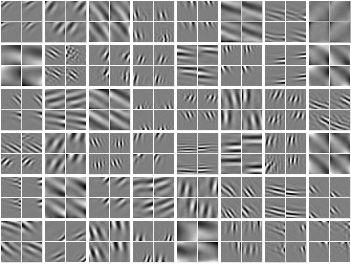
\includegraphics[scale=0.4]{SF_pool_SF.png}
\end{center} 
Fully connected $\rightarrow$ ReLU $rightarrow$ $L_2$-Pooling in non-overlapping groups of four 
\item Experiments with a standard convolutional network stage were performed. The architecture used was (1)convolution $\rightarrow$ (2)ReLU $\rightarrow$ (3)Volumetric Max-Pooling
\end{itemize}  
\begin{center}
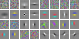
\includegraphics[scale=2]{dec2.png}
\end{center} 
Here is a 32-kernel filter bank consisting of 9x9 kernels. Every two horizontal neighbors constitute a max-pooling group (no overlap). Often semantically similar templates (cyan/red gradients for example) are pooled together.  \\
\noindent
\underline{Side Issues} 
\begin{itemize} 
\item Dead filters: Initialization with k-means does not help in the convolutional setting. I am not trying to manually detect "dead" filters and revive them manually reinitilizing with k-means. \\  
\end{itemize} 
\noindent
\underline{Experiments to Perform} 
\begin{itemize} 
\item Decoding from the pooling: In order to visualize the features in the input space a non-linear decoder can be trained. This is not just a way to visualize the feature space but also a validation that the features are information preserving. If this works, then joint training of encoder and non-linear decoder becomes an option, this would be the first demonstration of a principled non-linear decoder that I know of. We have already seen some success with K-means decoders and this would tie in nicely with Arthur \& Joan's recent work on phase recovery.  
\begin{center}
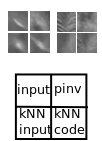
\includegraphics[scale=1.0]{example.png}
\end{center} 
\item Stacking and Training on Toy Data: I have not yet tried to train a second layer. 
\item Usefulness of the features: One approach is to show that features are useful in a standard classification task. This is problematic because few temporally coherent datasets contain labels (however NORB and COIL are exceptions). Furthermore very similar experiments have already been performed by in the ICML 2009 paper by Ronan Collobert and Jason Weston. In that work they actually put their own dataset together by photographing common objects in a studio environment and called it a COIL100-Like dataset. 
\end{itemize} 

  
\end{document} 